
\chapter{Planteamiento del proyecto}

En este cap\'\i tulo vamos a describir las ideas y contexto en el que vamos a desarrollar el contenido del proyecto.

\section{Descripci\'on}
Cuando un departamento de Recursos Humanos o una empresa de reclutamiento se enfrenta a una petici\'on para
cubrir un puesto vacante o de nueva creaci\'on, el proceso suele llevarse a cabo en diversas fases, que 
podr\'\i amos describir del siguiente modo \cite{proceso_seleccion1}:
\begin{enumerate}
\item {\bf Preselección}: etapa inicial en la que se detectan candidatos adecuados para el perfil buscado, bien recurriendo a 
anuncios en portales especializados, bien con b\'usquedas personalizadas de perfiles. En esta etapa se elabora una lista 
de candidatos que pasar\'an a las siguientes fases del proceso, descartando aquellos cuyas competencias no sean las adecuadas
para el puesto. 
\item {\bf Entrevista inicial}: en esta etapa los candidatos seleccionados en la etapa anterior son contactados para  
conseguir ampliar la informaci\'on de la que se dispone sobre ellos  (por ejemplo sobre las aptitudes
particulares y experiencias previas consignadas en el CV), y verificar el inter\'es y compromiso del candidato
con respecto a la oferta.
\item {\bf Informe}: tras la entrevista inicial, se seleccionan los mejores candidatos para el puesto, y se realiza un informe
donde se consignan los datos originales (el CV, por ejemplo) y los datos a\~nadidos en el curso de la entrevista inicial.
\item {\bf Presentaci\'on de candidatos}: el empleador recibe el informe elaborado en el punto anterior, y selecciona aquellos
que mejor se ajusten a sus necesidades, muy habitualmente realizando nuevas entrevistas con ellos.
\item {\bf Decisi\'on}: es el momento en que se elige el candidato al que se se le va a ofrecer el puesto, etapa en la 
que puede complementarse la informaci\'on recogida hasta el momento con referencias recabadas de anteriores empleadores.
\item {\bf Oferta}: etapa en la que la empresa presenta al candidato la oferta en firme, habitualmente por escrito, consignando 
la voluntad de la empresa de incorporar al candidato y los detalles econ\'omicos. 
\item {\bf Seguimiento}:  para comprobar que una vez incorporado a la empresa, tanto empleado como empleador est\'an conformes con
el resultado del proceso.
\end{enumerate}

Tradicionalmente, el comienzo de este proceso, la detecci\'on de candidatos, se realizaba en numerosas ocasiones 
a trav\'es de anuncios en prensa,
bases de datos de candidatos construidas a lo largo del tiempo, y la explotaci\'on de la red de contactos personales del entorno 
del empleador. Hoy por hoy, estos m\'etodos tradicionales han sido complementados, y algunos dir\'\i an que pr\'acticamente
suplantados, por m\'etodos que explotan la informaci\'on contenida en la web. 

Los t\'ecnicos de selecci\'on se enfrentan a un mundo muy diverso donde tanto la difusi\'on de los 
posibles puestos como la informaci\'on sobre los candidatos para los mismos est\'a diseminada en numerosos
formatos, teniendo un papel preponderante diversas plataformas o portales web (InfoJobs, Monster, etc.)
y redes sociales en general (LinkedIn, Twitter, Facebook, Instagram, etc.). Desde el punto de vista del t\'ecnico de selecci\'on, las
primeras contienen mucha informaci\'on sobre las aptitudes de los posibles candidatos, sus conocimientos, formaci\'on y 
experiencia, ya que son portales donde los propios usuarios consignan sus curricula vitae, y tambi\'en sobre su situaci\'on laboral
actual y expectativas. En el segundo grupo de fuentes, las redes sociales, hay algunas que tienen el car\'acter espec\'\i fico 
de las primeras (LinkedIn es el ejemplo m\'as claro), y hay otras en las que se consigna informaci\'on diversa, llam\'emoslas de 
prop\'osito general, tal vez en mayor medida personal que profesional.

El objetivo de nuestro proyecto es complementar el 
trabajo habitual de un departamento de Recursos Humanos o de un seleccionador de personal en
los portales y redes sociales dedicados al mundo laboral, con informaci\'on laboral extra\'\i da 
de fuentes menos est\'andar, como son las redes sociales de prop\'osito general. 
Estas redes son a menudo aprovechadas por los usuarios para difundir mensajes relacionados con su actividad
laboral, y una descripción de su actividad en las redes es relevante desde el punto de vista 
de un reclutador, en la medida que da informaci\'on del compromiso de la persona con su actividad, su valoración por
parte de otros usuarios, su proactividad, etc.

En este trabajo hemos elegido la red social Twitter por diversos motivos: es una red muy dinámica, fácil de usar, rápida y divertida,
que involucra cientos de millones de usuarios activos en todo el mundo: 328 millones según la web de la red. El crecimiento del número 
de usuarios fue casi exponencial entre 2010 y 2014, si bien últimamente la velocidad a la que adquiere nuevos usuarios ha perido intensidad.
Es también una red que, desde sus orígenes, ha puesto a disposición de los interesados los mecanismos necesarios para acceder a 
la información que atesora, con ciertas limitaciones, pero de forma relativamente sencilla. 



\myfigure{
\begin{tabular}{cc}
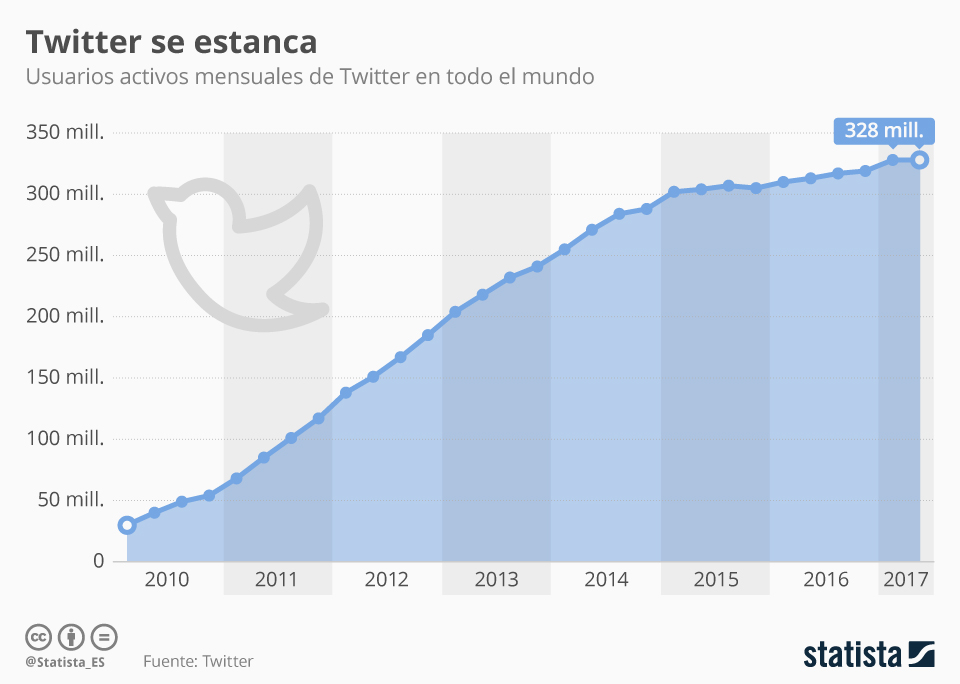
\includegraphics[width=0.4\textwidth]{usuarios_de_twitter}
&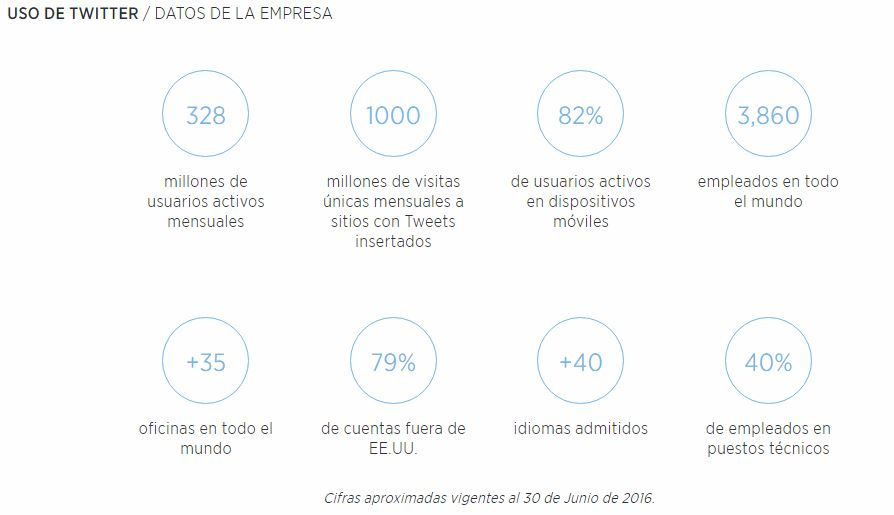
\includegraphics[width=0.4\textwidth]{twitter_uso_y_empresa}
\end{tabular}
\figcaption{Twitter: evolución del número de usuarios (Statista 2017, 
            \url{https://es.statista.com/grafico/10476/el-numero-de-usuarios-de-twitter-se-estanca })
			y datos de la empresa, \url{https://about.twitter.com/es/company }.}
\label{fig:Twitter_uso} }


Esta red da cabida a relaciones diversas, entre usuarios de variada índole. Dado que muchos de los usuarios 
publican información relacionada con su ocupación laboral, es natural esperar que en Twitter 
se formen comunidades de individuos que comparten interés en diferentes aspectos de dicho ámbito.
Nuestro propósito es definir e implementar un proceso que permita agregar información referente a 
esas comunidades a un determinado proceso de selección.

Observemos las dos siguientes ofertas de trabajo aparecidas recientemente (Septiembre 2017) en LinkedIn,
incluyendo los requisitos solicitados a los posibles candidatos:

\myfigure{\begin{tabular}{cc}
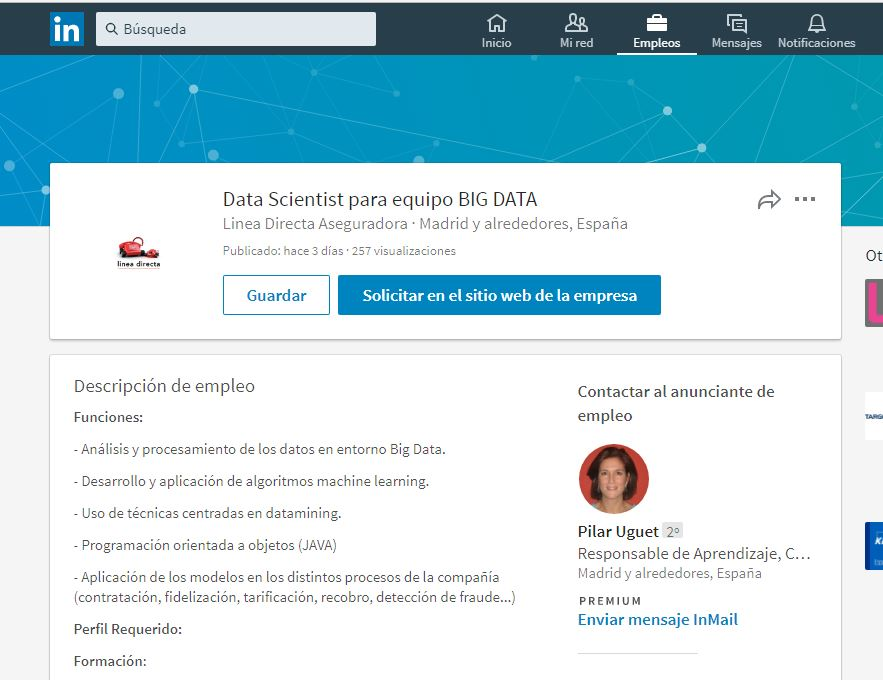
\includegraphics[width=0.4\textwidth]{oferta1_1}
&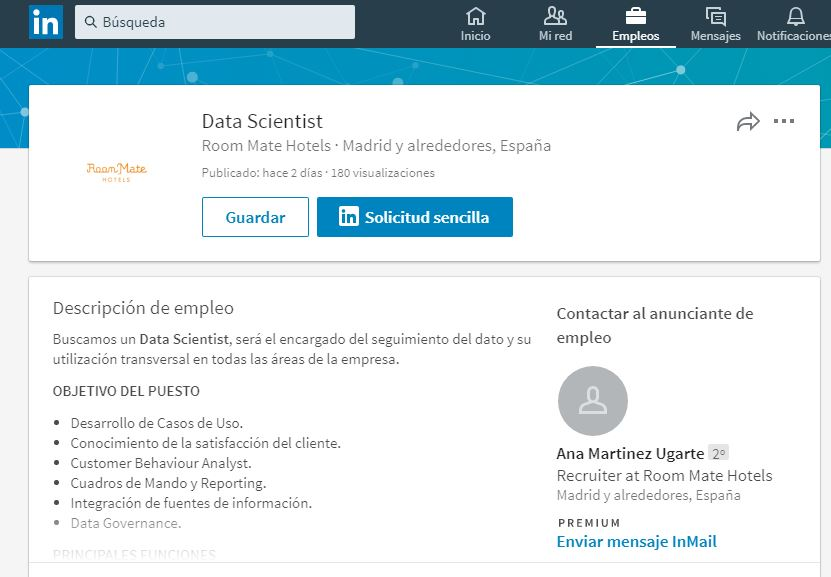
\includegraphics[width=0.4\textwidth]{oferta2_1}
\end{tabular}
\figcaption{Dos ofertas de empleo.}
\label{fig:ofertas_descripcion} }


\myfigure{\begin{tabular}{cc}
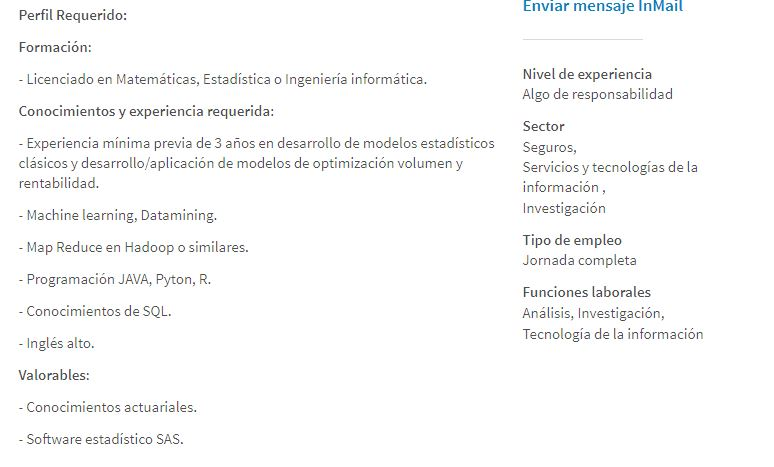
\includegraphics[width=0.4\textwidth]{oferta1_2}
&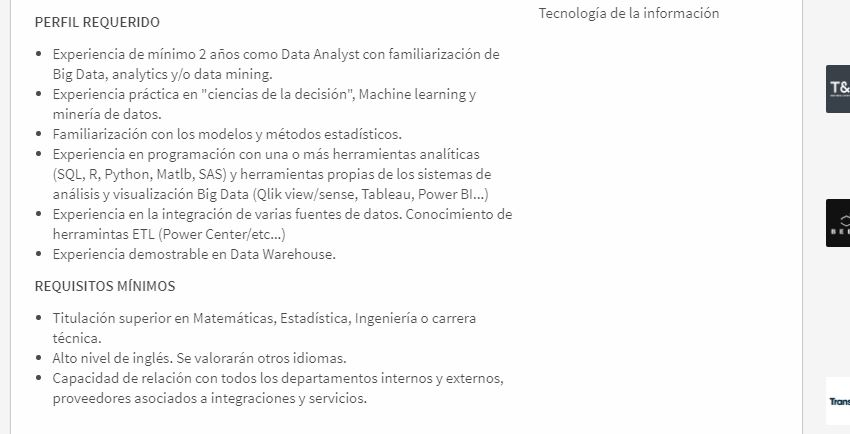
\includegraphics[width=0.4\textwidth]{oferta2_2}
\end{tabular}
\figcaption{Requisitos de las dos ofertas de empleo.}
\label{fig:ofertas_requisitos} }

En ambos casos, entre los requisitos se encuentran conocimientos sobre Python, R,
SQL, machine learning y data mining. Un reclutador probablemente usará esas palabras clave para buscar
los perfiles adecuados para alguno de los dos puestos, y construirá un conjunto de posibles candidatos (el
primer paso en nuestra descripción del proceso de contratación). En esta fase, y gracias a Octopus Data Insights,
nuestro reclutador contará con una ayuda extra. Octopus Data Insights le proporcionará una lista de usuarios
de Twitter que hayan publicado contenido en el que aparezcan esas palabras clave, que complementarán
el resultado que el reclutador haya obtenido por sus propios medios. La información proporcionada
por Octopus Data Insights resultará relevante también más adelante en el proceso,
cuando haya que tomar una decisión entre varios candidatos para determinar cuáles son los más adecuados para el 
puesto: usando la información de Twitter, los usuarios de la lista estarán ordenados según 
diversos criterios de relevancia.

El proceso para producir la información que ayudará al reclutador en el proceso es el siguiente:
\begin{enumerate}
\item Identificar los vocablos que determinan las habilidades que ha de poseer cualquier candidato
para la oferta en cuestión y extraer de Twitter aquellos tuits con contenido relacionado con ellos.
\item Dados esos tuits, construir un conjunto de usuarios, que entendemos como posibles candidatos 
a la oferta.
\item Usar la información publicada por los usuarios para determinar el grado de adecuación a la oferta
(serán más adecuados aquellos que hayan publicado información sobre todos los conocimientos requeridos que 
aquellos que solo hayan publicado sobre alguno de ellos, y más relevantes aquellos más activos, según el
número de tuits publicados sobre cada área).
\item Estudiar la relación entre los usuarios de este conjunto, y determinar los más relevantes en sentido
relativo (en términos de actividad en la red, cuáles son los más ``retuiteados", cuáles los más seguidos, etc.).
\end{enumerate}



\section{Contexto de negocio}
El área de Recursos Humanos de una compañía, incluso de una de las grandes\footnote{O
una empresa de {\em head hunting}, aunque en esta sección nos referimos solo a departamentos
de RRHH.}, no es el primer área 
en la que suele pensarse cuando hablamos de aplicaciones de las técnicas Big Data en el mundo
empresarial. En general,
parece difícil que los departamentos de RRHH de las compañías,  incluso de las mayores, produzcan
tradicionalmente tanta información propia como para necesitar el software y las herramientas especiales
que las técnicas Big Data proporcionan\footnote{\url{https://hbr.org/2017/06/theres-no-such-thing-as-big-data-in-hr }}:
muchas compañías tienen miles, no millones, de empleados, y la información que recogen con respecto a ellos
suele ser anual o cuatrimestral. En algunas ocasiones, el problema puede estar más incluso en
poder acceder a los datos de forma unificada (por el uso de distintos sistemas de almacenamiento),
y en entender y respetar las restricciones legales que aplican a los datos personales de los empleados
a la hora de manejarlos y trasladar los resultados a otros departamentos.

Desde que los primeros departamentos de Recursos Humanos aparecieron (en Estados Unidos
en los primeros años del siglo XX\footnote{\url{http://www.whatishumanresource.com/the-historical-background-of-human-resource-management }}),
se ha estudiado mucho la labor y la función de estos departamentos dentro de las organizaciones
empresariales, y las mejores técnicas y recursos para llevarlos a cabo, y existe abundante bibliografía
al respecto (ver, por ejemplo \url{http://www.whatishumanresource.com/hrm-text-books } para una
primera aproximación). Seguramente, la componente humana del profesional de RRHH no puede ser sustituida
en numerosas circunstancias. Sin embargo, el cambio que las tecnologías digitales
suponen en todos los ámbitos de la actividad humana sin duda impacta en las
actividades de los departamentos de RRHH. El principal uso del Big Data y del análisis
de datos debe ser la ayuda en la toma de decisiones, idealmente en todos los niveles
organizativos. Y es en los departamentos de RRHH donde se toman muchas decisiones sobre el
activo más valorable que compone las organizaciones: las personas.

Es por ello que el proceso de transformación digital de las empresas también
debiera incluir a los departamentos de Recursos Humanos, aprovechando los beneficios 
que les podría aportar un enfoque fundamentado en los datos para acometer su tarea.
Puede encontrarse abundante discusión en la red acerca del papel que las tecnologías y
técnicas Big Data pueden jugar en el área de RRHH\footnote{Entre muchos otros:

\noindent\url{https://www.business.com/articles/how-to-utilize-big-data-for-human-resources/ }, 

\noindent\url{https://blog.cake.hr/8-ways-use-hr-analytics-big-data-workplace/ }, 

\noindent\url{http://searchhrsoftware.techtarget.com/feature/Ready-or-not-here-comes-HR-analytics }, 

\noindent\url{https://www.forbes.com/sites/forbeshumanresourcescouncil/2017/02/02/six-powerful-ways-your-hr-team-can-leverage-big-data/\# 282624d65de9 }, 

\noindent\url{http://www.digitalistmag.com/future-of-work/2017/08/31/5-powerful-ways-hr-can-leverage-big-data-05242673 }, 

\noindent\url{https://www.villanovau.com/resources/hr/the-role-of-big-data-in-hr/\# .WkVNst_ibtQ }, 

\noindent\url{https://www.villanovau.com/resources/hr/big-data-changing-hr/\# .Wkdf39_ibtQ }, 

\noindent\url{https://www.cornerstoneondemand.com/glossary/big-data-hr }
} y también recientes estudios que intentan formalizar y dar contexto a dicho papel \cite{libro_rrhh}.
Entre otras, algunos de los aspectos de la labor de los departamentos de RRHH en los que
la aplicación de la tecnología Big Data puede ser de utilidad son los siguientes:
\begin{itemize}
\item \label{item:puntodeproyecto} Procesos de selección: incorporando datos de redes sociales y portales de empleo,
los procesos de selección pueden ser más específicos y eficientes en encontrar candidatos 
adecuados a las posiciones ofertadas. Este punto tiene gran importancia, puesto que
las pérdidas debidas a una mala contratación pueden ser cuantiosas\footnote{\url{https://www.entrepreneur.com/article/244730 }}.
\label{item:puntodeproyecto}

\item Factores de calidad en la contratación: las técnicas Big Data pueden ayudar a los profesionales de
RRHH a determinar qué factores en la trayectoria de un posible candidato son o no importantes a 
la hora de valorar su adecuación a un puesto dado y su rendimiento posterior. A veces, factores que
en principio pueden percibirse como muy importantes (años de experiencia pasada, si esa experiencia fue
en puestos similares o no,\dots) pueden en realidad ser irrelevantes a la luz de los datos disponibles
en la compañía (y cada una, en cada sector y momento, es distinta).

\item Formación y evaluación: no se trata solo de contratar a los mejores candidatos, sino
de que las personas se adapten pronto a sus nuevas labores y al nuevo entorno de trabajo,
y mantener una continua formación que permita al trabajador adaptarse a los cambios en dicho
entorno. Con las técnicas de análisis de datos, puede ser más fácil decidir qué formación es 
la más adecuada para cada profesional, y evaluar los beneficios de dicha formación.

\item Retención de los empleados: evaluando el historial de la compañía,
las técnicas de análisis de datos pueden ayudar a identificar las causas por las que un empleado
deja de formar parte de la misma. A partir de ahí, se pueden identificar aquellos que no 
permanecerán en la compañía, así como aquellos factores que mejor funcionan para retener a los empleados,
y potencialmente optimizar el uso de los recursos destinados a fidelización de empleados. 
Medir la percepción de la sociedad de la compañía como lugar de trabajo a través de las impresiones
reflejadas en redes sociales, por ejemplo, también puede ayudar a los profesionales de RRHH a
identificar áreas de mejora o áreas a potenciar,
a la hora de atraer candidatos para nuevos puestos y retener a los trabajadores.

\item Medida del desempeño: las técnicas de análisis de datos también pueden ayudar a medir
el desempeño de los empleados de forma más precisa, por ejemplo determinando la relación entre 
franjas horarias trabajadas y rendimiento, identificando a los trabajadores más productivos de
forma absolutamente objetiva, o llevando a cabo evaluaciones del desempeño
más frecuentes que anualmente o trimestralmente. Otro aspecto importante en este punto es el uso de dispositivos 
encaminados a monitorizar la actuación de los trabajadores: por ejemplo, plataformas de escucha 
{\em online} para seguir en tiempo real el desempeño en un {\em call center}, o ayudar a los trabajadores
en el trascurso de su quehacer. Este tipo de dispositivos también puede ayudar a los departamentos
de RRHH a cuidar estrechamente la seguridad del trabajador, el cumplimiento de las políticas
de buenas prácticas, etc.

\item Compensación monetaria: el dinero que ganan los empleados con su trabajo es el
factor básico de la satisfacción del empleado. Usando el análisis de datos, los equipos de 
RRHH pueden desarrollar un modelo financiero optimizado. Esto es especialmente importante
en compañías grandes, con empleados en distintas geografías, donde resulta difícil comparar 
los distintos departamentos internacionales. Y es importante en cualquier compañía tener
una guía de cómo realizar una promoción adecuada de los trabajadores optimizando
los costes asociados.

\item Planificación: el análisis de datos puede ayudar a las compañías a identificar tendencias y 
planificar acciones. Por ejemplo, se pueden detectar épocas de mayor absentismo por cuestiones de 
salud e implementar políticas para paliarlo (de prevención sanitaria o de contratación de refuerzos), o 
detectar factores que conducen a una mayor incidencia de accidentes que pueden afectar a la producción
y programar acciones para remediarlo.

\end{itemize}

En general, el uso de técnicas de análisis de datos y Big Data, ayudará a cambiar el enfoque
de los departamentos de RRHH a un papel más proactivo, y a ampliar el rango de herramientas en las
que apoyarse al tomar decisiones.

El abanico de aplicaciones enfocadas a la gestión de Recursos humanos es bastante amplio
(en \url{https://www.capterra.com/human-resource-software/ } podemos encontrar una lista con
varias aplicaciones y soluciones enfocadas a este tema), y van desde soluciones propuestas
por proveedores generales de tecnología Big Data y análisis de datos,
como las de Oracle y SAP, a sistemas propuestos por proveedores más especializados, 
como SumTotal Systems, PeopleFluent, Cornerstone, Talent Analytics, CakeHR.
Algunas compañías han desarrollado soluciones propias,
por ejemplo el {\em Project Oxygen} de Google, enfocada a evaluar la actividad de los managers y 
ayudarlos en su desempeño.

Nuestro proyecto se encuadra dentro del primer punto mencionado en la página 
\pageref{item:puntodeproyecto}, y el objetivo es, como ya se ha mencionado,
ayudar en la labor de localizar candidatos a un puesto de trabajo
a través de la extracción y análisis de información de Twitter.
Es por tanto un proyecto que clasificará perfiles de usuarios de Twitter.


Varios  trabajos han explorado la clasificación de usuarios de Twitter
atendiendo a su actividad (ver \cite{tesis_mariluz} y las referencias
incluidas, \cite{user_class5}), para descubrir 
características de usuarios como etnia o género(\cite{user_class1}, \url{https://www.kaggle.com/crowdflower/twitter-user-gender-classification }),
para clasificar la orientación política (\cite{user_class2}) o 
detectar usuarios similares adecuados para seguir (\cite{user_class3}),
detección de bots (\cite{user_class4}), 
entre otros enfoques.
 

En cuanto a aplicaciones que extraigan información de Twitter y proporcionen 
algún tipo de clasificación de usuarios, podemos encontrar una amplia variedad.
Algunas de las más comentadas en la red son las siguientes:
\begin{itemize}
\item StatusPeople.com: analiza los seguidores de una cuenta de Twitter y los clasifica como buenos, malos o inactivos.
\item Mentionmapp: crea un mapa interactivo que dibuja por menciones, la interacción de una cuenta de Twitter con las últimas 200 publicaciones de la cuenta. Sirve para determinar la calidad de la audiencia en Twitter y poder detectar y diferenciar entre seguidores, fans y superfans.
\item Audiense (antes SocialBro): es una herramienta para identificar audiencias relevantes (de dónde proceden los followers, en qué idioma escriben, si sus cuentas son públicas o privadas, si son cuentas verificadas, identifica seguidores inactivos, etc.). También examina el contenido psicolingüístico de los tuits y permite a las marcas conocer los rasgos de personalidad que están detrás del comportamiento de compra de los usuarios.
\item Twitter Audit: analiza una cuenta tomando como referencia 5.000 seguidores del usuario y le asigna una puntuación según el número de tuits, la fecha del último tuit y la proporción de seguidores/seguidos. Y a continuación, asigna un porcentaje de \lq\lq veracidad\rq\rq de los seguidores de dicha cuenta.
\item Untweeps: averigua qué seguidores de una cuenta no han tuiteado en los últimos 30 días, y facilita dejar de seguirles.
\item Followerwonk: busca usuarios por palabras clave en sus biografías de los usuarios y los muestra por orden de influencia, pudiendo filtrar por localización, número de followers, número de Tweets, etc. 
\item Buzzsumo: esta herramienta sirve para localizar usuarios influyentes en Twitter a partir de palabras clave o para medir el rango de influencia de una persona o marca en concreto. 
\item Klear: también para localizar usuarios influyentes en diversas plataformas, además de Twitter.
\item Trolldor: ofrece una lista negra de cuentas de Twitter clasificadas como falsos usuarios influyentes o trolls.
\item Klout: puntúa el perfil social según su influencia y facilita una lista de las bios más influyentes según la temática. Propone contenidos para mejorar la puntuación de una cuenta.
\item Peerindex: también ayuda a encontrar usuarios influyentes, en diversas redes sociales además de Twitter.
\end{itemize}

Hasta donde conocemos, no hay ninguna aplicación, comercial o no, 
ni trabajo académico, que tenga la misma orientación que el proyecto 
que desarrollamos. Hay, por supuesto, referencias en las que nos apoyaremos
para clasificar el lenguaje de los tuits y descripciones, para determinar qué perfiles
son personas, y para clasificar el texto de los tuits, así como para luego ordenar
por importancia y relevancia los usuarios detectados (de todas estas referencias hablaremos
más concretamente en cada punto particular). Sin embargo, 
la combinación de técnicas que proponemos en este proyecto no la hemos encontrado,
y en particular, no la hemos encontrado enfocada al objetivo planteado: encontrar
posibles candidatos relevantes para una oferta de trabajo a partir de
la actividad relacionada en Twitter.



\section{Objetivos y criterio de éxito}
Como hemos mencionado anteriormente, nuestro objetivo final es proporcionar una lista de usuarios de Twitter que hayan publicado contenido relacionado con una oferta de trabajo, ordenados por relevancia, de forma que un reclutador pudiera usarla para contactar con ellos e incluirlos en su proceso de selección.

Nuestro criterio de éxito es por tanto conseguir dicha clasificación de los usuarios,
y aportar valor con un método propio, particularizable y eficiente, para conseguirlo. 

\section{Hip\'otesis y limitaciones}
La hipótesis fundamental que estamos haciendo al iniciar este proceso, es que la actividad en Twitter
acerca de un determinado tema (por ejemplo, publicar algo relacionado con Python), supone
que el usuario en cuestión tiene conocimientos sobre dicho tema (en nuestro caso, entenderíamos que ese
usuario posee conocimientos de Python). Esto es cuestionable, por supuesto, pero también ponderable
si tenemos en cuenta que la actividad no sea esporádica. Si un usuario publica sobre un tema
en numerosas ocasiones, la hipótesis de que ese tema no le resulta ajeno, va cobrando fuerza.

Entre las limitaciones de las que adolece el proceso definido para llevar a cabo el proyecto, se encuentran las 
siguientes:
\begin{enumerate}
\item En general, no todos los posibles candidatos tienen por qué usar Twitter, y por tanto habrá muchos que 
queden directamente fuera de nuestro proceso.
\item Los tuits utilizados en el proceso están sujetos a una ventana temporal. Habrá muchos candidatos,
usuarios de Twitter, que no aparezcan en nuestros registros, por no presentar actividad durante ese tiempo.
\item Twitter impone limitaciones en la cantidad de información a la que deja acceder, y por ello, también es
posible que los usuarios pierdad visibilidad en este proceso, 
porque el contenido publicado por ellos no se encuentre entre el proporcionado por la red social durante el proceso
de extracción de datos.
\end{enumerate}


Otra limitación del proceso es que la información que obtenemos de la red es a nivel de usuario de Twitter. 
La dirección de correo o el nombre verdadero de la persona en cuestión, o cualquier dato que pudiera identificarla
no está necesariamente disponible en la aplicación, salvo que el usuario lo haya querido hacer público explícitamente. 
Esta información, y la forma en que se utilice, es clave para la usabilidad del resultado del proyecto, en dos aspectos principales:
\begin{enumerate}
\item para que el reclutador pueda hacer uso de la información, la persona ha de estar identificada, lo suficientemente
como para abrir un canal de comunicación entre el reclutador y el posible candidato.
\item Desde el punto de vista de la comercialización del resultado del proyecto, el hecho de identificar usuarios en una red
social y usar esa información con fines lucrativos, ha de ser implementado de forma muy cuidadosa. El impacto de la Ley 
Orgánica de Protección de Datos de Carácter Personal (LOPD) es muy relevante en nuestro proyecto, y merece un apartado especial.
Nos ocupamos de ello en la sección \ref{subsection:LOPD}.
\end{enumerate}
En relación al primer punto, evidentemente proporcionar un usuario de Twitter ya es abrir un canal de
comunicación. Sin embargo, solo la información de las publicaciones del usuario no es suficiente para 
incluirlo en un proceso de selección, incluso antes del primer contacto entre reclutador y candidato,
y el primero probablemente  necesitará más información (por ejemplo un CV) para considerar al segundo. 
Una forma de solventarlo sería cruzar la información de Twitter (el nombre de usuario)
con la contenida en otros portales (como LinkedIn,  Facebook, Academia.edu, ResearchGate, Glassdoor, etc.),
ya que a menudo el usuario de Twitter es parte de los datos consignados en los CV. Esta extensión
del proyecto la hemos dejado deliberadamente fuera del planteamiento de este proyecto, aunque sería 
{\em conditio sine qua non} para una implementación comercializable del proyecto.




\subsection{La Ley Orgánica 15/1999, de 13 de diciembre, de Protección de Datos
de Carácter Personal}
\label{subsection:LOPD}

La Agencia Española de Protección de Datos, AEDP, define un dato de carácter personal del siguiente modo:

\myfigure{
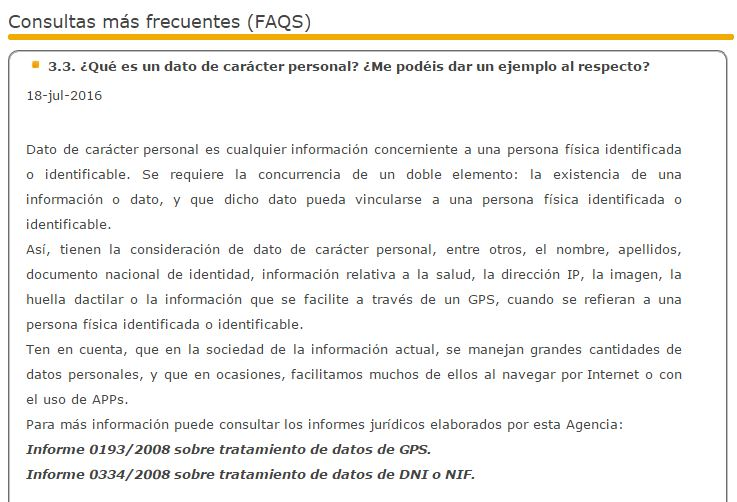
\includegraphics[width=0.6\textwidth]{dato_personal}
\figcaption{AEDP preguntas frecuentes,
           \url{https://sedeagpd.gob.es/sede-electronica-web/vistas/infoSede/detallePreguntaFAQ.jsf;jsessionid=147951A8A98D206E87F2655B9E96E7EB?idPregunta=FAQ%2F00025%
		   }} 
\label{fig:dato_personal} }

El perfil en Twitter de un usuario se puede considerar por tanto un dato de carácter personal, en tanto en cuanto
permitiría localizar e identificar al usuario, tal vez a través de cruces de la información en Twitter con
información adicional (por ejemplo, lo que comentábamos a propósito de encontrar el CV del usuario usando que
frecuentemente, el usuario de Twitter es parte de la información contenida en el mismo, y el CV está disponible en otros 
portales). Sin embargo, en la política de privacidad de Twitter (\url{https://twitter.com/es/privacy })
se establece que
\begin{center}
\noindent\begin{minipage}{0.9\linewidth}%{0.9\columnwidth}
\centering%
{\em ''Al utilizar cualquiera de nuestros Servicios, usted da su consentimiento para la recopilación, 
 la transferencia, la manipulación, el almacenamiento, la revelación y otros usos de su información 
 según lo descrito en esta Política de Privacidad. Esto incluye cualquier información que elija proporcionar que 
 se considere sensible según la legislación vigente."}
\end{minipage}
\end{center}
Y también, en relación a la información del perfil o publicaciones:
\begin{center}
\noindent\begin{minipage}{0.9\linewidth}%{0.9\columnwidth}
\centering%
{\em ''{\bf Información básica de la cuenta}: si opta por crear una cuenta de Twitter, debe promocionar cierta información personal, 
como su nombre, nombre de usuario, contraseña, dirección de correo electrónico o número de teléfono. 
En Twitter, su nombre y nombre de usuario siempre se hacen públicos, incluso en su página de perfil y en los resultados de búsqueda, 
y puede utilizar su nombre real o un seudónimo."

''{\bf Tuits, gente que sigue, listas, perfil y otra información pública}: Twitter está principalmente diseñado para ayudarle a 
compartir información con el mundo. La mayoría de la información que usted nos facilita a través de Twitter es información 
que nos está pidiendo que hagamos pública. Puede facilitarnos información de perfil para hacerla pública en Twitter, como por 
ejemplo, una breve biografía, su ubicación, su sitio web, fecha de nacimiento, o una fotografía. Además, su información pública 
incluye los mensajes que tuitea; los metadatos facilitados con los tuits, tales como cuándo ha tuiteado y la aplicación cliente 
que utilizó para tuitear; información sobre su cuenta, como el momento de su creación, el idioma, el país y la zona horaria; y las 
listas que crea, las personas a las que sigue, los tuits que retuitea o marca como Me gusta, y las emisiones de Periscope en las que 
hace clic o con las que se relaciona de alguna forma (por ejemplo, haciendo comentarios o clic en el icono de corazón) en Twitter. 
Twitter disemina amplia e instantáneamente su información pública a una amplia gama de usuarios, clientes y servicios, incluyendo 
motores de búsqueda, desarrolladores y editores que integran contenido de Twitter en sus servicios y organizaciones, tales como universidades, 
agencias de salud pública y empresas de investigación de mercado que analizan la información en busque de tendencias y conocimiento."}
\end{minipage}
\end{center}
A tenor de estas afirmaciones, la información que nosotros vamos a manejar en la implementación de este proyecto
(nombre de usuario, información del perfil, tuits publicados)
es una información de carácter público. 

En su enunciado, la LOPD establece que
(texto extraído del informe jurídico  2013-0184 de la AEPD
\url{http://www.agpd.es/portalwebAGPD/canaldocumentacion/informes_juridicos/otras_cuestiones/common/pdfs/2013-0184_Red-social-y-creaci-oo-n-de-perfiles-de-empleados..pdf%
})
\begin{center}
\noindent\begin{minipage}{0.9\linewidth}%{0.9\columnwidth}
\centering%
{\em Establece a este
respecto la Ley Orgánica 15/1999 en su artículo 2 que ''El régimen de
protección de los datos de carácter personal que se establece en la
presente Ley Orgánica no será de aplicación: a) A los ficheros
mantenidos por personas físicas en el ejercicio de actividades
exclusivamente personales o domésticas."
}
\end{minipage}
\end{center}

Y define las actividades personales a continuación:

\begin{center}
\noindent\begin{minipage}{0.9\linewidth}%{0.9\columnwidth}
\centering%
{\em
En cuanto a la determinación de que se entiende por actividades
personales o domésticas dispone el Reglamento de desarrollo de la LOPD en
su artículo 4 que ''Sólo se considerarán relacionados con actividades
personales o domésticas los tratamientos relativos a las actividades que se
inscriben en el marco de la vida privada o familiar de los particulares."
Esta es también la interpretación del término ''personal" contenida en la
Sentencia de la Audiencia Nacional de 15 de junio de 2006 al señalar que ''(…)
Será personal cuando los datos tratados afecten a la esfera más íntima de la
persona, a sus relaciones familiares y de amistad y que la finalidad del
tratamiento no sea otra que surtir efectos en esos ámbitos.

También dará lugar a la aplicación de la Ley Orgánica 15/1999, por
superar el ámbito de la vida privada o familiar de los particulares la publicación
de datos de terceros en la red cuando no existan limitaciones de acceso a su
perfil, en cuanto que dicha publicación constituye una cesión de datos, definida
en el artículo 3 j) de la LOPD como “Toda revelación de datos realizada a una
persona distinta del interesado”, ya que en estos supuestos, como señalaba la
sentencia la Sentencia de 6 de noviembre de 2003 (caso Bodil Lindqvist) del
Tribunal de Justicia de las Comunidades Europeas, no se inscribe en el marco
de la vida privada o familiar de los particulares “un tratamiento de datos
personales consistente en la difusión de dichos datos por Internet de modo que
resulten accesibles a un grupo indeterminado de personas.”}
\end{minipage}
\end{center}




Refiriéndose incluso a datos de carácter público que aparecen en los datos,
la interpretación de la LOPD respecto al uso de los mismos por terceros, especialmente
en el caso en el que la finalidad de dicho uso sea comercial, es que el único medio
para legitimar el uso es el consentimiento explícito de la persona cuyos datos van 
a utilizarse. Este consentimiento ha de cumplir unas determinadas condiciones
(de nuevo extraemos del informe jurídico  2013-0184 de la AEPD)
\begin{center}
\noindent\begin{minipage}{0.9\linewidth}%{0.9\columnwidth}
\centering%
{\em 
El tratamiento de datos de carácter personal debe encontrarse fundado
en alguna de las causas legitimadoras previstas en el artículo 6 de la Ley
Orgánica 15/1999, disponiendo a este respecto su número primero que ''El
tratamiento de los datos de carácter personal requerirá el consentimiento
inequívoco del afectado, salvo que la ley disponga otra cosa."

(\dots)

Dicho
consentimiento debe reunir las características señaladas en el
artículo 3.h de la misma Ley que lo define como ''manifestación de
voluntad, libre, inequívoca, específica e informada, mediante la que el
interesado consienta el tratamiento de datos personales que le
conciernen".

Esta Agencia ha venido describiendo en sus informes dichas
características de manera que se entiende por consentimiento libre aquel que
ha sido obtenido sin la intervención de vicio alguno del consentimiento en los
términos regulados por el Código Civil.
}
\end{minipage}
\end{center}


\myfigure{
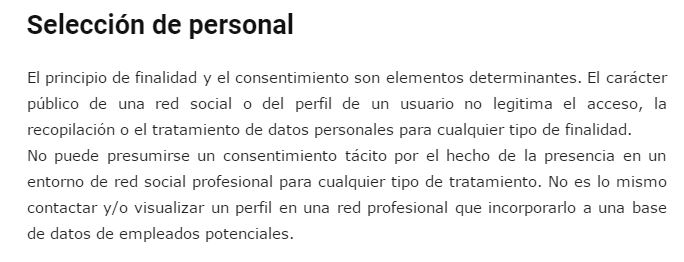
\includegraphics[width=0.6\textwidth]{LOPD1}
\figcaption{Ayuda Ley de Protección de Datos, 
           \url{https://ayudaleyprotecciondatos.es/2010/09/16/redes-sociales-empresas-y-proteccion-de-datos/ }}
\label{fig:LOPD1} }


Como consecuencia de toda esta información, entendemos lo siguiente:
\begin{itemize}
\item que los datos del perfil de los usuarios de Twitter, así como sus publicaciones en dicha red,
tienen carácter público.
\item Que el carácter público de dichos datos no es óbice para poder manipularlos y distribuirlos
a terceros, en ninguna actividad que no se circunscriba al ámbito personal o familiar.
\item La elaboración de un proyecto de fin de máster no tiene por qué entenderse como una 
actividad del ámbito personal o familiar, con lo cual no estaría en disposición de difundir esa información
a terceros, salvo en las condiciones previstas en la LOPD.
\item Cualquier versión comercializable de este proyecto debería contar con los mecanismos
adecuados para obtener el consentimiento explícito de los usuarios para el uso de sus perfiles, 
y posible inclusión en un proceso de selección de personal. Esta fase quedará fuera del plan de elaboración
del proyecto.
\end{itemize}
% Para eliminar el riesgo relativo a protección de datos en la elaboración del proyecto, 
% pero sin alterar su esencia, proponemos publicar los resultados enmascarando los nombres 
% de usuario de aquellos que aparezcan en nuestra base de datos.

\section{Esquema de desarrollo del proyecto}
En las siguientes secciones de la memoria iremos estudiando y describiendo las distintas
fases que componen el proyecto, que podemos dividir en tres grandes subgrupos:
\begin{enumerate}
\item Comenzaremos por hacer un análisis descriptivo de la base de datos recogida a partir del API de Twitter, en relación con el problema que nos ocupa. Estudiaremos la proporción de tuits originales
frente a retuiteados, número de tuits descargados por día, número de retuits, relación entre el 
número de tuits descargados y el número de usuarios distintos, el número de tuits por usuario, y
los hastags presentes en los mensajes. Esta tarea la llevaremos a cabo en el capítulo \ref{chap:tratamiento_inicial_de_los_datos}.

\item A continuación, comienza la fase de proceso de la información. Nuestro objetivo es 
constuir una lista de usuarios que podamos recomendar a un profesional de Recursos Humanos como
posibles candidatos para una oferta. El primer paso, realizado en el capítulo \ref{chap:extraccion_de_usuarios}, es entonces seleccionar, a partir de la información descargada de Twitter, los usuarios de interés. 

\item La fase final será, con esa lista de usuarios extraídos en la fase anterior, ordenarlos
en función de su comportamiento en Twitter. La metodología empleada en este apartado, así como una descripción de los resultados, se abordan en el capítulo \ref{chap:ordenacion_de_usuarios}.
\end{enumerate}